\documentclass[tikz,crop,convert={density=200,outext=.png},border=0.4cm]{standalone}

\usepackage{pgfplots}
\usepackage{amsmath}
\usetikzlibrary{arrows.meta}
\usepackage{physics}
\usepackage{xcolor}
\definecolor{mixed_1}{RGB}{8,48,107}
\pgfplotsset{compat=newest,
    %width=6cm,
    %height=3cm,
    scale only axis=true,
    max space between ticks=25pt,
    try min ticks=5,
    every axis/.style={
        axis y line=middle,
        axis x line=middle,
        axis line style={thick,->,>=latex, shorten >=-.3cm}
    },
    every axis plot/.append style={thick},
    tick style={black, thick},
}
\tikzset{
    semithick/.style={line width=0.8pt},
}
\usepgfplotslibrary{groupplots}
\usepgfplotslibrary{dateplot}
% Document begins
\begin{document}
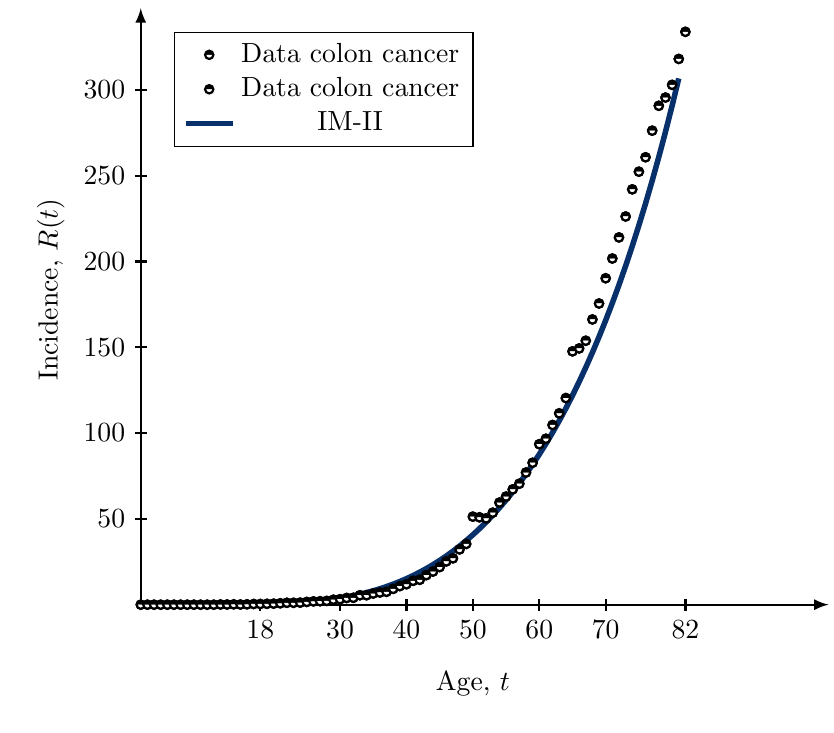
\begin{tikzpicture}
  % The axis of the plot
\begin{axis}[
    %title={Model: $\dv{y}{t}=\frac{2y}{t}$ with solution $y(t)=C_1t^2$\\Symmetry: $\Gamma_{\epsilon}=(t,y)\mapsto\left(\exp\left(\epsilon\right)t,\exp\left(-\epsilon\right)y\right)$},
    title style = {align=left},
    xlabel={Age, $t$},
    ylabel={Incidence, $R(t)$},
    %ylabel={Logarithm of Incidence, $\ln\left(R(t)\right)$},    
    % ylabel={Incidence, $R(t)$},
    x label style={at={(axis description cs:0.5,-0.1)},anchor=north},
    y label style={at={(axis description cs:-0.1,0.55)},rotate=90,anchor=south},    
    % xmin=-27, xmax=5,
    % xmin=0, xmax=82.5,
    xmin=0, xmax=100,    
    xtick={0,18,30,40,...,60,70,82},    
    %ymin=-20, ymax=20,
    %xtick={-30,-27,...,9},
    %ytick={-15,-10,...,15},
    legend style={at={(axis description cs:0.05,0.9)},anchor=west},    
    %legend pos=north west,
    %ymajorgrids=true,
    grid style=dashed,
]
% Plot the data
\addplot[
only marks, mark=halfcircle*,mark size=1.5pt,color=black,
]
coordinates {%
(0.0,0.0)
(1.0,0.0)
(2.0,0.0)
(3.0,0.0)
(4.0,0.0)
(5.0,0.0)
(6.0,0.0)
(7.0,0.0)
(8.0,0.0)
(9.0,0.0)
(10.0,0.0)
(11.0,0.0)
(12.0,0.1)
(13.0,0.1)
(14.0,0.2)
(15.0,0.1)
(16.0,0.2)
(17.0,0.4)
(18.0,0.4)
(19.0,0.5)
(20.0,0.6)
(21.0,0.8)
(22.0,1.1)
(23.0,1.1)
(24.0,1.2)
(25.0,1.6)
(26.0,1.9)
(27.0,2.0)
(28.0,2.2)
(29.0,2.9)
(30.0,3.2)
(31.0,3.9)
(32.0,4.0)
(33.0,5.5)
(34.0,5.5)
(35.0,6.5)
(36.0,7.1)
(37.0,7.5)
(38.0,9.2)
(39.0,10.8)
(40.0,11.9)
(41.0,13.9)
(42.0,14.5)
(43.0,17.2)
(44.0,19.3)
(45.0,21.9)
(46.0,25.2)
(47.0,27.0)
(48.0,32.2)
(49.0,35.4)
(50.0,51.3)
(51.0,50.9)
(52.0,50.3)
(53.0,53.6)
(54.0,59.5)
(55.0,63.0)
(56.0,67.2)
(57.0,70.5)
(58.0,77.0)
(59.0,82.7)
(60.0,93.5)
(61.0,96.7)
(62.0,104.7)
(63.0,111.5)
(64.0,120.4)
(65.0,147.6)
(66.0,149.3)
(67.0,153.8)
(68.0,166.2)
(69.0,175.5)
(70.0,190.2)
(71.0,201.7)
(72.0,214.0)
(73.0,226.2)
(74.0,242.0)
(75.0,252.3)
(76.0,260.7)
(77.0,276.2)
(78.0,290.7)
(79.0,295.5)
(80.0,302.9)
(81.0,318.0)
(82.0,333.8)
};
\addlegendentry{Data colon cancer}
\addplot[
only marks, mark=halfcircle*,mark size=1.5pt,color=black,
]
coordinates {%
(0.0,0.0)
(1.0,0.0)
(2.0,0.0)
(3.0,0.0)
(4.0,0.0)
(5.0,0.0)
(6.0,0.0)
(7.0,0.0)
(8.0,0.0)
(9.0,0.0)
(10.0,0.0)
(11.0,0.0)
(12.0,0.1)
(13.0,0.1)
(14.0,0.2)
(15.0,0.1)
(16.0,0.2)
(17.0,0.4)
(18.0,0.4)
(19.0,0.5)
(20.0,0.6)
(21.0,0.8)
(22.0,1.1)
(23.0,1.1)
(24.0,1.2)
(25.0,1.6)
(26.0,1.9)
(27.0,2.0)
(28.0,2.2)
(29.0,2.9)
(30.0,3.2)
(31.0,3.9)
(32.0,4.0)
(33.0,5.5)
(34.0,5.5)
(35.0,6.5)
(36.0,7.1)
(37.0,7.5)
(38.0,9.2)
(39.0,10.8)
(40.0,11.9)
(41.0,13.9)
(42.0,14.5)
(43.0,17.2)
(44.0,19.3)
(45.0,21.9)
(46.0,25.2)
(47.0,27.0)
(48.0,32.2)
(49.0,35.4)
(50.0,51.3)
(51.0,50.9)
(52.0,50.3)
(53.0,53.6)
(54.0,59.5)
(55.0,63.0)
(56.0,67.2)
(57.0,70.5)
(58.0,77.0)
(59.0,82.7)
(60.0,93.5)
(61.0,96.7)
(62.0,104.7)
(63.0,111.5)
(64.0,120.4)
(65.0,147.6)
(66.0,149.3)
(67.0,153.8)
(68.0,166.2)
(69.0,175.5)
(70.0,190.2)
(71.0,201.7)
(72.0,214.0)
(73.0,226.2)
(74.0,242.0)
(75.0,252.3)
(76.0,260.7)
(77.0,276.2)
(78.0,290.7)
(79.0,295.5)
(80.0,302.9)
(81.0,318.0)
(82.0,333.8)
};
\addlegendentry{Data colon cancer}

% Plot the model
\addplot[
color=mixed_1,line width=2pt,
]
coordinates {%
(18.0,0.28975529392760097)
(19.0,0.3790054022898802)
(20.0,0.49013510644939834)
(21.0,0.6270028113293583)
(22.0,0.7938254429420968)
(23.0,0.9951601799388687)
(24.0,1.2358800190079249)
(25.0,1.5211442719397832)
(26.0,1.856365306296367)
(27.0,2.2471729674152114)
(28.0,2.699378154683985)
(29.0,3.218936975193656)
(30.0,3.811916774972599)
(31.0,4.484465168410258)
(32.0,5.2427829688770515)
(33.0,6.093101686849071)
(34.0,7.041666023472428)
(35.0,8.094721562123581)
(36.0,9.258507659321808)
(37.0,10.539255366779265)
(38.0,11.943190082308663)
(39.0,13.476538529511059)
(40.0,15.145539602910992)
(41.0,16.956458582980037)
(42.0,18.915604219666868)
(43.0,21.02934819848959)
(44.0,23.30414653476705)
(45.0,25.74656248431225)
(46.0,28.363290608580986)
(47.0,31.161181685237704)
(48.0,34.147268208474124)
(49.0,37.3287902749951)
(50.0,40.713221699818746)
(51.0,44.308296249919316)
(52.0,48.122033922728605)
(53.0,52.16276723041282)
(54.0,56.43916747974517)
(55.0,60.96027106156222)
(56.0,65.73550578363016)
(57.0,70.77471729670945)
(58.0,76.08819567619729)
(59.0,81.68670223143623)
(60.0,87.58149662207613)
(61.0,93.78436436620511)
(62.0,100.30764482871793)
(63.0,107.16425978090938)
(64.0,114.3677426238747)
(65.0,121.9322683692199)
(66.0,129.87268447104793)
(67.0,138.20454260337)
(68.0,146.94413147714147)
(69.0,156.10851079114934)
(70.0,165.71554641108142)
(71.0,175.78394687135224)
(72.0,186.33330129470588)
(73.0,197.38411882529797)
(74.0,208.9578696719131)
(75.0,221.0770278592149)
(76.0,233.765115786477)
(77.0,247.04675069509963)
(78.0,260.9476931484053)
(79.0,275.49489762970705)
(80.0,290.7165653674756)
(81.0,306.6421994995855)
};
\addlegendentry{IM-II}

\end{axis}
\end{tikzpicture}

\end{document}
